\documentclass[10pt,a4paper]{article}
\usepackage[utf8x]{inputenc}
\usepackage{ucs}
\usepackage{amsmath}
\usepackage{amsfonts}
\usepackage{amssymb}
\usepackage{a4wide}
\usepackage{comment}
\usepackage[pdftex]{graphicx}
\usepackage{epstopdf}
\newcommand{\cmd}[1]{\texttt{#1}}
\newcommand{\remove}{}
\newcommand{\dir}[1]{\textsf{#1}}
\newcommand{\pop}{Depiler\xspace}
\newcommand{\push}{Empiler\xspace}
\newcommand{\tete}{LireTete}
\newcommand{\sommet}{LireSommet}
\newcommand{\empt}{EstVide}
\newcommand{\enqueue}{Enfiler\xspace}
\newcommand{\dequeue}{Defiler\xspace}
\newcommand{\get}{\ensuremath{\leftarrow\ }}

\usepackage[textsize=small, textwidth=2cm, color=yellow]{todonotes}


\usepackage{comment}
\usepackage{algorithm}
\usepackage[noend]{algpseudocode}
\usepackage{tcolorbox}

\newtcolorbox{mybox}[3][]
{
  colframe = #2!25,
  colback  = #2!10,
  coltitle = #2!20!black,  
  title    = {#3},
  #1,
}


\excludecomment{solution}
\includecomment{solution}

\title{IF111 - Algorithmes et structures de données-TD3 :\\ Graphes et représentations}
\date{}
\author{\underline{Jonathan Narboni}, Rohan Fossé}
\date{\underline{\texttt{jonathan.narboni@labri.fr}}, \texttt{rfosse@labri.fr}}


\begin{document}
\maketitle

\section*{Exercice 1}
\begin{figure}[h]
    \centering
    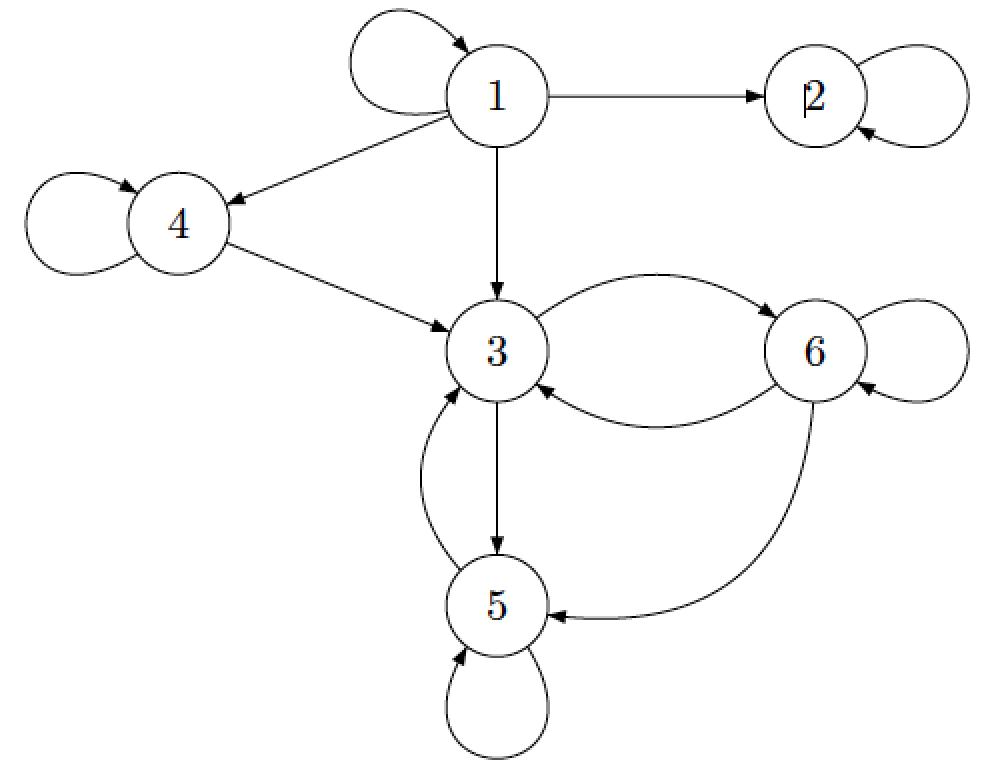
\includegraphics[scale=0.3]{Graphe1.png}
    \label{fig:my_label}
\end{figure}
\begin{enumerate}
    \item Donner une représentation du graphe ci-dessus au moyen d'une liste d'adjacence, puis au moyen d'une liste d'incidence.
    \item Donner maintenant une représentation du même graphe en matrice d'incidence, Quels problèmes rencontre-t-on ?
    \item Proposer un algorithme de construction de la matrice d'incidence à partir de la liste d'adjacence d'un graphe, puis à partir de sa matrice d'adjacence,
\end{enumerate}


\section*{Exercice 2}
Considérons un graphe orienté $G = (V, E)$. Un sommet $v$ est un \textit{puits universel} s'il est de degré entrant $|V| - 1$ et de degré sortant 0.
Étant donnée une représentation d'un graphe $G = (V, E)$ par une matrice d'adjacence, proposer un algorithme permettant de déterminer s'il existe un puits universel.

\begin{tcolorbox}
 i est un puits universel si et seulement si dans la matrice la ligne i ne contient que
des 0 et la colonne i ne contient que des 1 sauf à l’intersection de la ligne i. On peut donc tester de façon exhaustive, ce qui prend un temps quadratique en fonction de $|V|$.
\end{tcolorbox}

\section*{Exercice 3}
Un passeur se trouve au bord d'une rivière avec un loup, une chèvre et une salade. Comme vous le savez probablement, les loups mangent les chèvres mais pas les salades, les chèvres mangent les salades mais pas les loups, et les salades ne mangent personne. Dans sa barque, le passeur ne peut transporter qu'un seul des trois protagonistes à la fois. Lorsqu'il est dans sa barque ou sur la rive opposée, il ne peut empêcher le carnage, On souhaite savoir s'il peut amener, sains et saufs, de l'autre coté de la rive le loup, la chèvre et la salade.
Si cela est possible, combien de traversées sont nécessaires ?\\
Pour répondre à ce problème, vous donnerez une modélisation par un graphe.

\begin{tcolorbox}
\begin{itemize}
    \item P = Passeur; C = Chèvre; L = Loup; S = Salade
    \item Lettre sur une arête = un trajet en barque
    \item - : Passeur qui fait trajet seul
\end{itemize}
\end{tcolorbox}
\begin{figure}
    \centering
    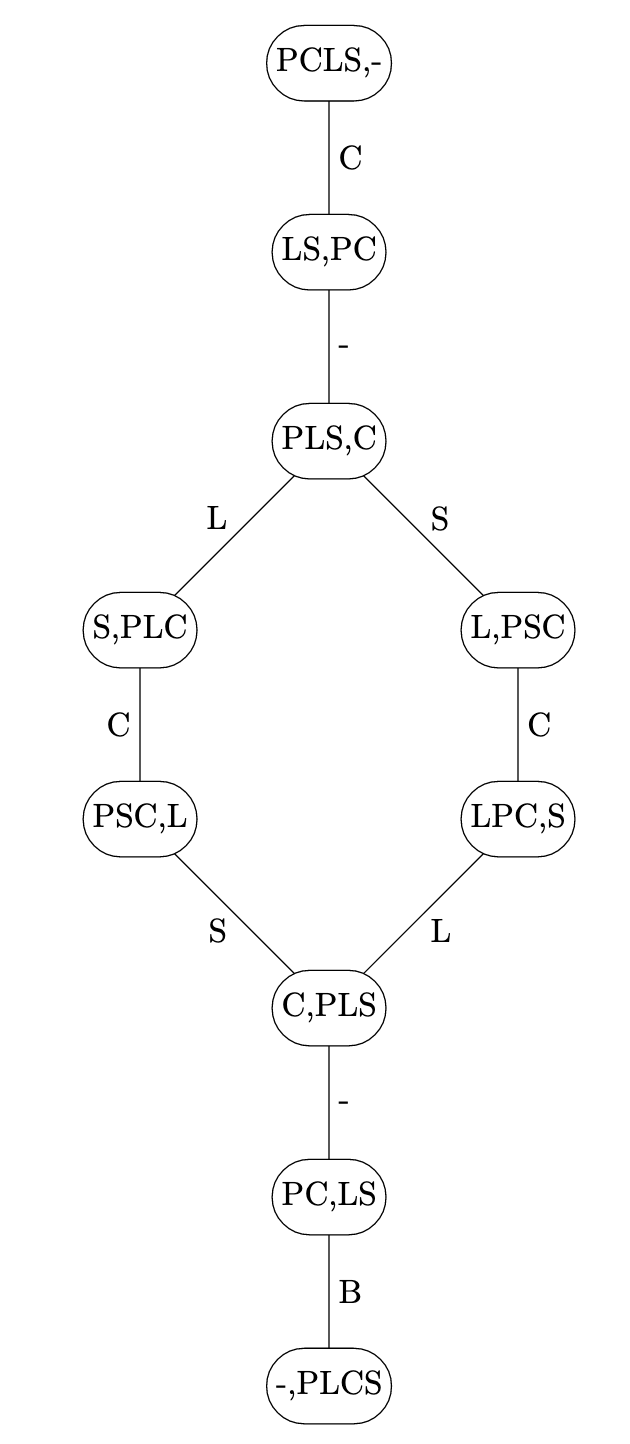
\includegraphics[scale=0.5]{passeur.png}
    \caption{Correction de l'exercice 3}
    \label{fig:my_label}
\end{figure}


\section*{Exercice 4}

Tout graphe contenant un triangle ($K_3$) ne peut être colorié en moins de trois couleurs.

\begin{enumerate}
    \item Construire un graphe sans triangle qui nécessite également trois couleurs.
    \item Comment construire un graphe sans $K_4$ nécessitant 4 couleurs ?
    \item un graphe sans $K_5$ nécessitant 5 couleurs ?
\end{enumerate}

\begin{tcolorbox}
Il suffit de considérer par exemple un cycle ayant un nombre impair de sommets. Si l’on rajoute à ce graphe un sommet relié à tous les sommets du cycle, on obtient un graphe de nombre chromatique 4 ne contenant pas de K4. On peut itérer cette construction de façon à obtenir, pour tout k, un graphe de nombre chromatique k ne contenant pas de Kk. Un résultat plus puissant, dû à Erdös, montre que pour tout k, il existe un graphe de nombre chromatique k sans triangle, et même sans cycle de longueur inférieure à un entier p donné, quel que soit p…
\end{tcolorbox}

\end{document}

